
%%%%
%%
%% This file sets up the Sign and Label datatypes and creates Sign and
%% Label macros.
%%
%% Signs generally represent interesting parts of game area, usually
%% as things posted on walls.  Labels represent other things, often on
%% or inside envelopes, that are part of complex mechanics.
%%
%% The default value for \MYloc will inherit location from the Place
%% or Sign most immediately up the ownership tree.  Override this by
%% setting \MYloc to anything (even blank).
%%
%% Sign is for full-sized signs that would cover most of a large
%% manila envelope; SignMedium is for signs sized to half-sized manila
%% envelopes; SignSmall is for signs sized for small manila envelopes
%% (the same size as item cards).  Label, LabelMedium, and LabelSmall
%% are analagous, but they don't have a \takedownby note at the
%% bottom.  You can always use a sign or label without an envelope or
%% with a differently-sized envelope.  Choose which based on
%% visibility and content.
%%
%% SignTiny is for signs you want to be hard to find; it is small and
%% does not have a \takedownby note.  SignDot is for a very small
%% "dot" which only has a title.
%%
%% SignStrip produces a strip of paper (without a \takedownby note)
%% with labels on the outside that show on both sides if you fold it
%% in half.  These are a convenient alternative to sub-envelopes. They
%% can also be used for "s-packets" taped to walls (see
%% Extras/README-s-packets).
%%
%% LabelCover produces a label similar to the cover to a research
%% notebook.  LabelPage, likewise, produces a page.
%%
%% EOG is for full-sized end-of-game signs.
%%
%%%%%

\DECLARESUBTYPE{Sign}{Element}
\PRESETS{Sign}{
  \FD\MYloc	{\mylocation} %% real-space location
  \FD\MYtext	{} %% text of sign
  }
\POSTSETS{Sign}{
  \edef\mylocation{\MYloc}
  \protected@edef\@ownerstring{%
    \MYname%
    \ifx\mylocation\empty\else\ (\mylocation)\fi%
    }
  }
\def\mylocation{}

\def\loc#1{\rs\MYloc{#1}}

\DECLARESUBTYPE{SignMedium}{Sign}
\DECLARESUBTYPE{SignSmall}{Sign}
\DECLARESUBTYPE{SignTiny}{Sign}
\DECLARESUBTYPE{SignDot}{Sign}
\PRESETS{SignDot}{\s\MYtext{}}

\DECLARESUBTYPE{Label}{Sign}
\PRESETS{Label}{\s\MYloc{}}
\DECLARESUBTYPE{LabelMedium}{Label}
\DECLARESUBTYPE{LabelSmall}{Label}

\DECLARESUBTYPE{SignStrip}{Sign}
\DECLARESUBTYPE{LabelCover}{Label}
\DECLARESUBTYPE{LabelPage}{Label}

\DECLARESUBTYPE{EOG}{Sign}
\PRESETS{EOG}{%
  \s\MYname	{End Of Game}
  \s\MYtext	{{\bf\Huge You may not pass through here.}}
  }


%%%%%
%% \signbig[<location>]{<name>}{<text>}
%% \eog[<location>]
%%
%% \signmdeium[<location>]{<name>}{<text>}
%% \signsmall[<location>]{<name>}{<text>}
%% \signtiny[<location>]{<name>}{<text>}
%% \signdot[<location>]{<name>}
%%
%% \labelbig{<name>}{<text>}
%% \labelmedium{<name>}{<text>}
%% \labelsmall{<name>}{<text>}
%%
%% \signstrip[<location>]{<name>}{<text>}
%% \labelcover{<name>}{<text>}
%% \labelpage{<name>}{<text>}
\newinstance{Sign}{\signbig[3][\mylocation]}{
  \s\MYloc{#1}\s\MYname{#2}\s\MYtext{#3}}
\newinstance{EOG}{\eog[1][\mylocation]}{\s\MYloc{#1}}

\newinstance{SignMedium}{\signmedium[3][\mylocation]}{
  \s\MYloc{#1}\s\MYname{#2}\s\MYtext{#3}}
\newinstance{SignSmall}{\signsmall[3][\mylocation]}{
  \s\MYloc{#1}\s\MYname{#2}\s\MYtext{#3}}
\newinstance{SignTiny}{\signtiny[3][\mylocation]}{
  \s\MYloc{#1}\s\MYname{#2}\s\MYtext{#3}}
\newinstance{SignDot}{\signdot[2][\mylocation]}{
  \s\MYloc{#1}\s\MYname{#2}}

\newinstance{Label}{\labelbig[2]}{
  \s\MYname{#1}\s\MYtext{#2}}
\newinstance{LabelMedium}{\labelmedium[2]}{
  \s\MYname{#1}\s\MYtext{#2}}
\newinstance{LabelSmall}{\labelsmall[2]}{
  \s\MYname{#1}\s\MYtext{#2}}

\newinstance{SignStrip}{\signstrip[3][\mylocation]}{
  \s\MYloc{#1}\s\MYname{#2}\s\MYtext{#3}}
\newinstance{LabelCover}{\labelcover[2]}{
  \s\MYname{#1}\s\MYtext{#2}}
\newinstance{LabelPage}{\labelpage[2]}{
  \s\MYname{#1}\s\MYtext{#2}}


%%%%%
%% \sEOG{}
%% use \sEOg[\loc{<location>}]{} for EOG sign at a specific place
\NEW{EOG}{\sEOG}{
  }


%%%%%%%%%%%%%%%%%%%%%%%%%%%%%%%%%%%%%%%%%%%%%%%%%%%%%%%%%%%%%%%%%%


\NEW{Sign}{\sPRHolder}{
  \s\MYname	{Press Releases}
 % \s\MYloc	{10-250}
  \s\MYtext	{Get a Press Release form from here if you need one.}
  \s\MYwhites	{\multi{10}{\wPressRelease{}}}
}

\NEW{Sign}{\sLivingRoom}{
  \s\MYname	{Living Room}
 % \s\MYloc	{10-250}
  \s\MYtext	{A moody but artistic living room with lots of art and uncomfortable leather furniture.}
  }
  
 \NEW{Sign}{\sLair}{
  \s\MYname	{Basement}
 % \s\MYloc	{10-250}
  \s\MYtext	{A forbidding and dark Villaincave.}
  }
  
  \NEW{Sign}{\sComputer}{
  \s\MYname	{Computer}
 % \s\MYloc	{10-250}
  \s\MYtext	{A shiny gadget.}
  }
 
  \NEW{Sign}{\sWallPhone}{
  \s\MYname	{WallPhone}
  %\s\MYloc	{10-250}
  \s\MYtext	{A vintage dial phone.}
  } 
  
    \NEW{Sign}{\sBullets}{
  \s\MYname	{Field of Bullets}
 % \s\MYloc	{10-250}
  \s\MYtext	{A field of bullets fire as soon as you enter the room.
If you have an item with number \iBulletproofCape{\MYnumber}, nothing happens.
If you have an item with number \iFancyUtilityBelt{\MYnumber}, you are wounded for 1 minute.
If you don't have either item, you are wounded for 5 minutes.
}
  } 
  
      \NEW{Sign}{\sHQ}{
  \s\MYname	{Phone}
%  \s\MYloc	{10-250}
  \s\MYtext	{A regular phone to be used on urgent calls.}
  } 
  
       \NEW{Sign}{\sNewsReports}{
  \s\MYname	{Hero PR Level}
 % \s\MYloc	{10-250}
  \s\MYtext	{An indication of the League of Heroes Public Relations status.}
  } 
  
       \NEW{Sign}{\sChrisSign}{
  \s\MYname	{Try Me}
 % \s\MYloc	{10-250}
  \s\MYtext	{It's \cChrisHemsworth{\intro}! His entire body is encased in a solid cube of steel. He's trying to tell you something through the gag in his mouth.
		Go fetch a GM.}
  } 
  
        \NEW{Sign}{\sArtRoom}{
  \s\MYname	{Gallery}
 % \s\MYloc	{10-250}
  \s\MYtext	{A gallery of rare and valuable artwork that \cGrandma{\intro} has acquired.}
  } 
  
        \NEW{Sign}{\sComputerRoom}{
  \s\MYname	{Computer Room}
 %\s\MYloc	{10-250}
  \s\MYtext	{Come here for your Internet needs.}
  } 
  
        \NEW{Sign}{\sDiningRoom}{
  \s\MYname	{Dining Room}
  %\s\MYloc	{10-250}
  \s\MYtext	{There is a table full of delicious food.  \cGrandma{\MYsupername}'s minions constantly refill emptied plates.}
  } 
  
   \NEW{Sign}{\sLairDoor}{
  \s\MYname	{A Door}
% \s\MYloc	{10-250}
  \s\MYtext	{There is a door here that looks as if it was newly installed.}
  }
  
     \NEW{Sign}{\sGrandmaArt}{
  \s\MYname	{1962}
%  \s\MYloc	{10-250}
  \s\MYtext	{The artist and the audience are just two sides of the same coin.}
  }
  
     \NEW{Sign}{\sClue}{
  \s\MYname	{Instructions}
%  \s\MYloc	{10-250}
  \s\MYtext	{Steal the \iBagofHolding{} that belongs to \cOS{} and bring it to me. The first person who presents it to me will win the grand prize!\\
{\em If you are not one of \cGrandma{}'s grandchildren, this is completely uninteresting.}
}

 \NEW{Sign}{\sArtOneImage}{
  \s\MYname	{One}
 % \s\MYloc	{10-250}
  \s\MYtext	{a}
 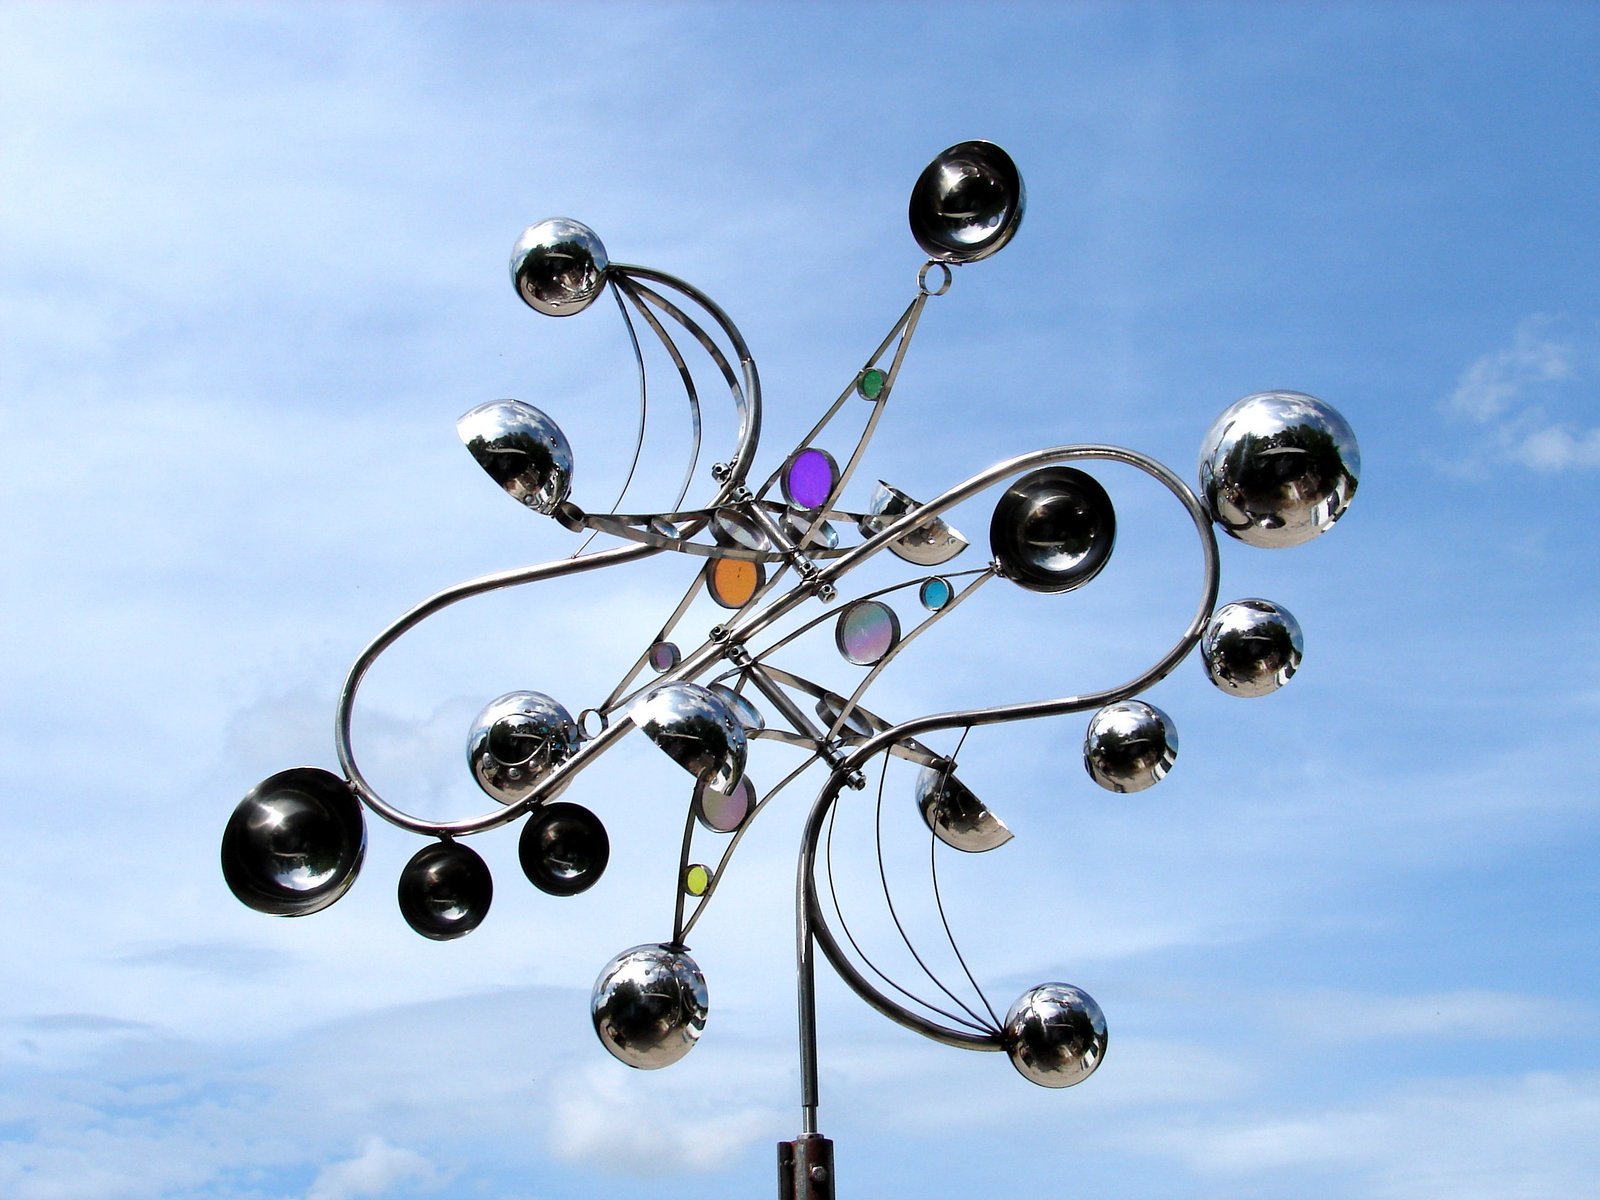
\includegraphics[width=0.8\textwidth]{ArtworkOne.png}
  }
  
  \NEW{Sign}{\sArtTwoImage}{
  \s\MYname	{Two}
 % \s\MYloc	{10-250}
  \s\MYtext	{a}
 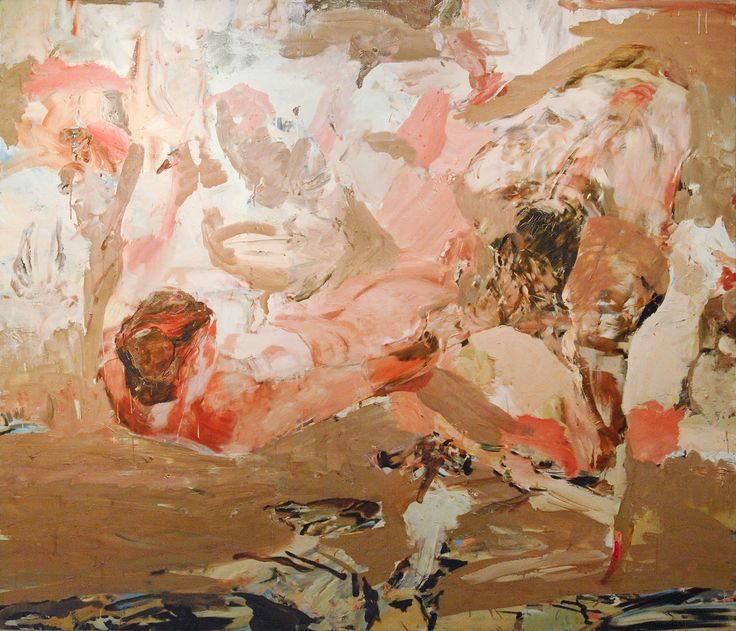
\includegraphics[width=0.8\textwidth]{ArtworkTwo.png}
  }
  
   \NEW{Sign}{\sArtThreeImage}{
  \s\MYname	{Three}
  %\s\MYloc	{10-250}
  \s\MYtext	{a}
 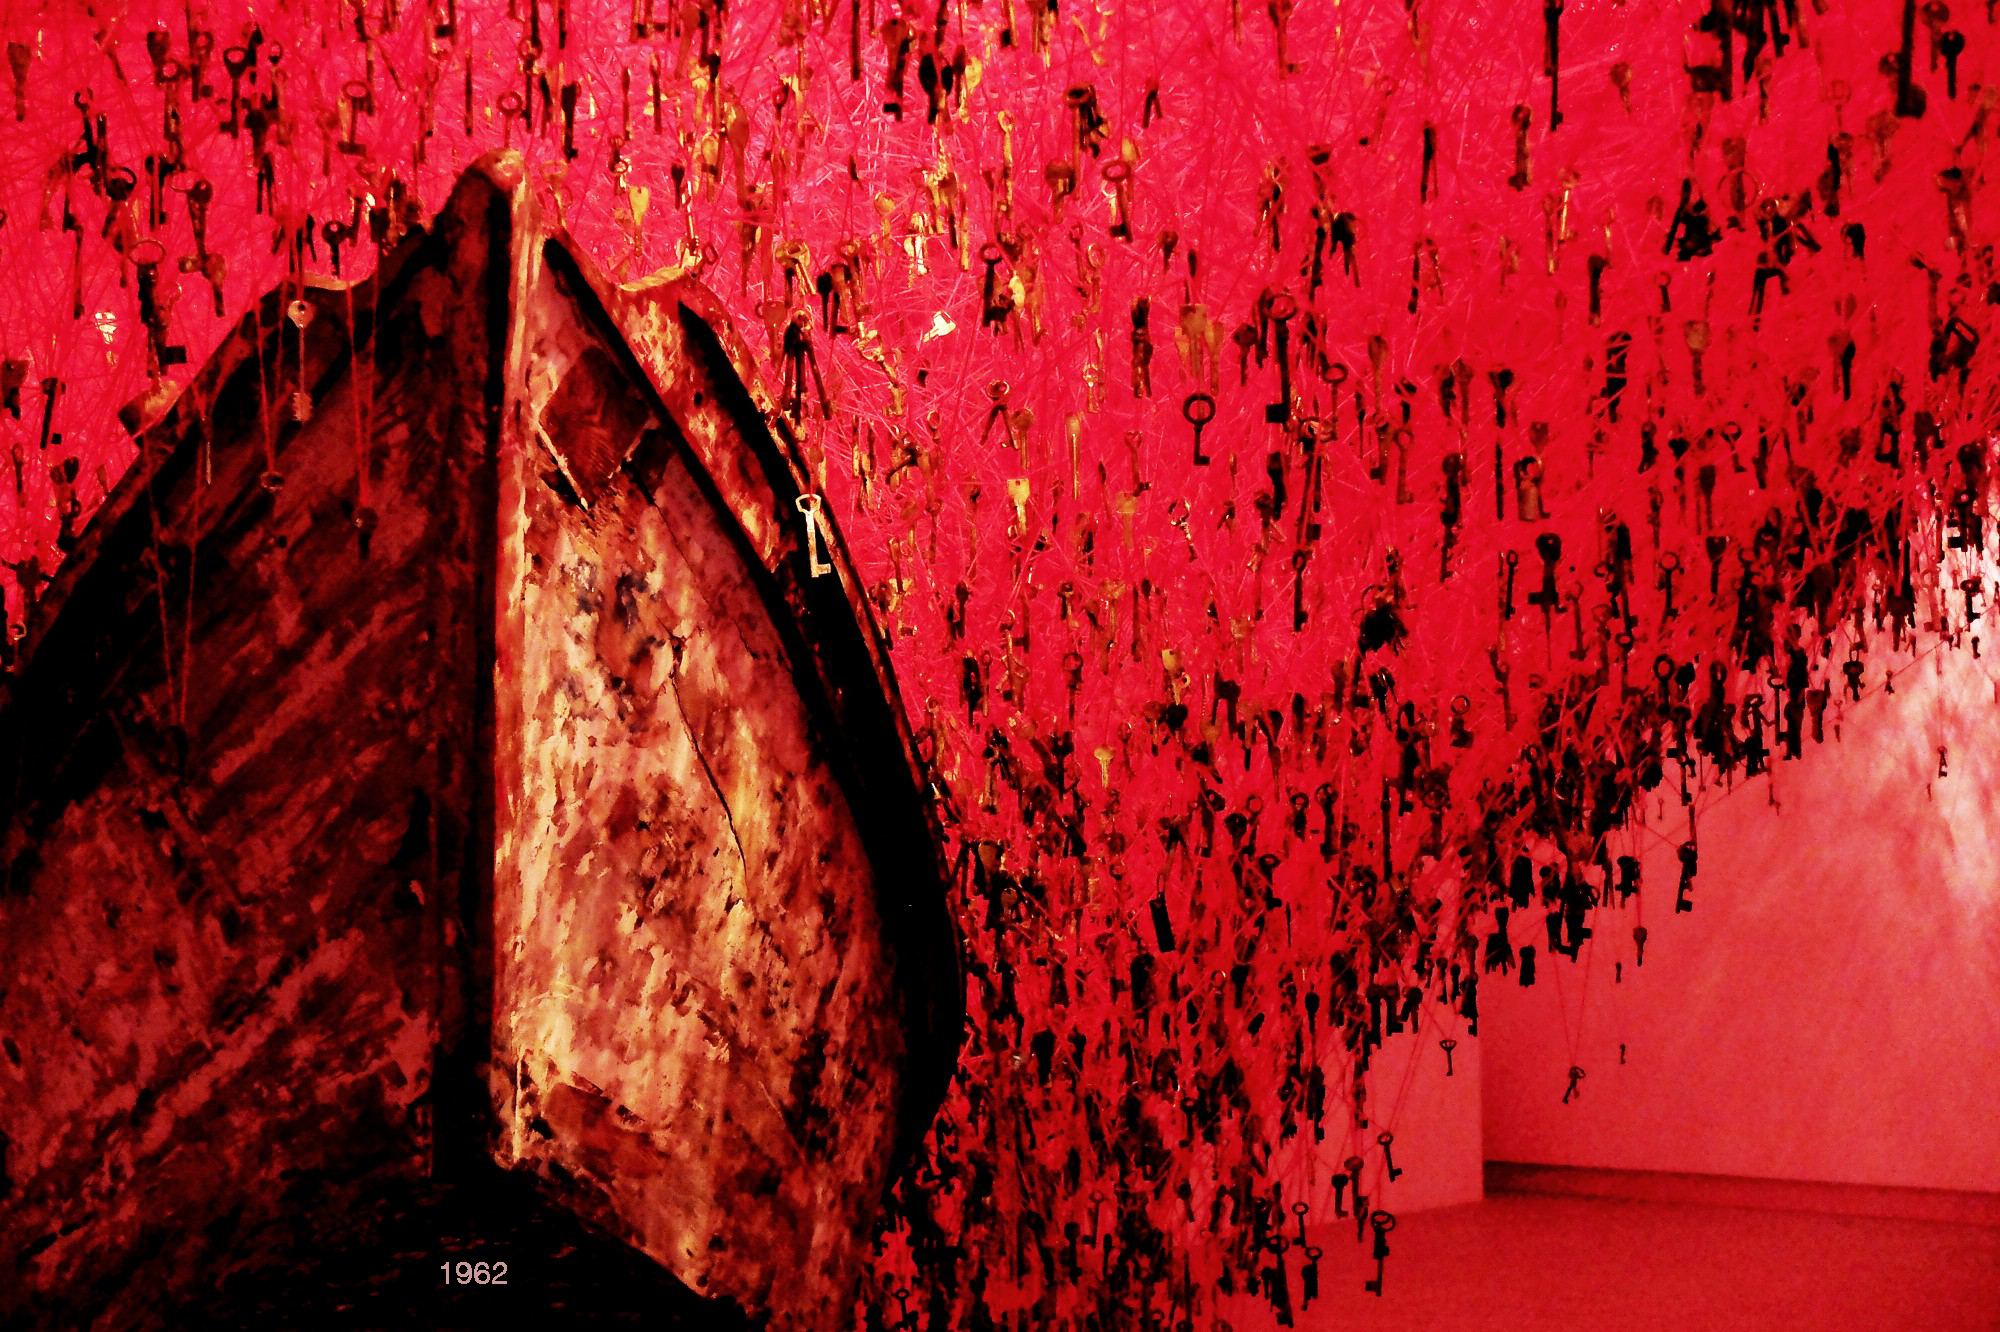
\includegraphics[width=0.8\textwidth]{ArtworkThree.png}
  }
  
  }

%%%%%%%%%%%%%%%%%%%%%%%%%%%%%%%%%%%%%%%%%%%%%%%%%%%%%%%%%%%%%%%%%%
